% Chapter Template

\chapter{Software Framework} % Main chapter title

\label{Chapter4} % Change X to a consecutive number; for referencing this chapter elsewhere, use \ref{ChapterX}

\lhead{Chapter 4. \emph{Software Framework}} 
		The ROS\cite{quigley2009ros} is the de facto standard used for any robotics related research in the recent times. However it is officially supported only for the Ubuntu distribution which makes it unavailable to the people who work with sensors that are being support only for Windows system (i.e Kinect for windows v2). Hence a distributed architecture which is not specific to any operating system or programming language is proposed which uses open network communication standards and transparent message passing using structured data. In this chapter the design philosophy of the software framework and core components of the system are explained.
		
\section{Framework Design}		
	The system could contain nodes/processes which can be running in the same computer or might be running anywhere in the network. The order of start and stop of these nodes essentially do not matter.
\subsection{Communication Protocol}	
	The nodes communicate with each other as shown in Fig~\ref{fig:framework} using either inproc/IPC/TCP/UDP protocols depending on its location and to whom it wants to communicate with. The communication between the nodes is established using ZeroMQ\cite{ZeroMQ} library which has a variety of advantages any modern application would require like  
\begin{itemize}
\item Multiple language and Cross platform
\item Message using inproc,IPC,TCP,UDP protocols
\item Support for patterns like Publisher-Subscriber, Push-Pull, Request-Response
\item Tiny and high-speed asynchronous implementation
\end{itemize}
	ZeroMQ comes with the low-level C API. High-level bindings exist in 40+ languages including Python, Java, PHP, Ruby, C, C++, C\#, Erlang, Perl, and more. So it can run in literally any OS and owing to its very low memory foot print it can also run on the mobile devices and tablets.
\begin{figure}
\centering
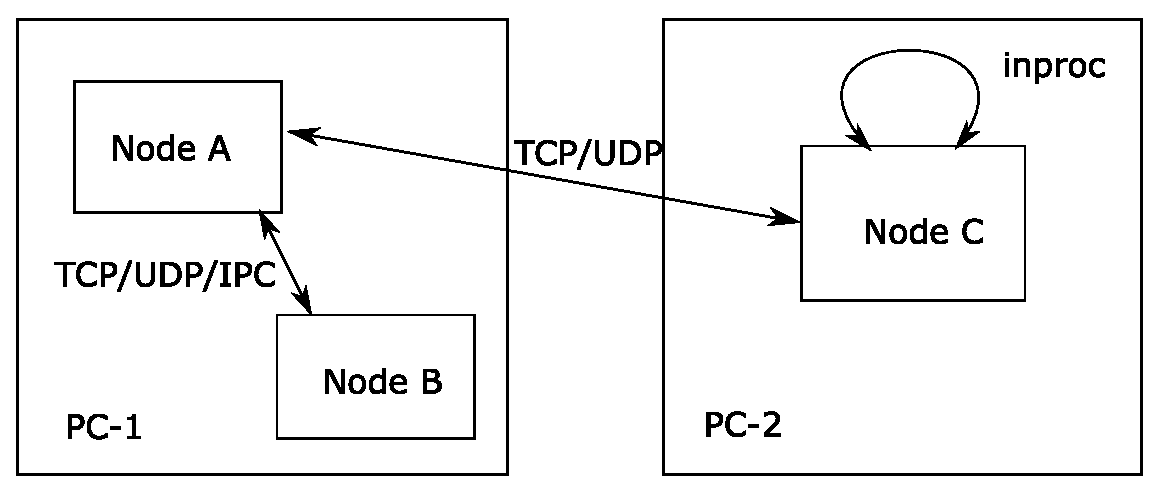
\includegraphics[width=\textwidth]{assets/architecture_comm.eps}
\caption[Framework Communication Protocol]{Framework Communication Protocol}
\label{fig:framework}
\end{figure}
\subsection{Message Format}
	The nodes communicate with each other using structured data formatted using the Google Protocol buffers\cite{ProtocolBuffers}. Protocol buffers are Google's language-neutral, platform-neutral, extensible mechanism for serializing structured data. It could be thought of as XML format, but smaller, faster, and simpler. The data could be structured once as per the requirement, then the special generated source code could be integrated with the application to easily write and read structured data to and from a variety of data streams and using a variety of languages – Java, C++, C\# or Python. The message is defined in a file with extension *.proto which will be consumed by the code generator to generate code for a specific language. A sample proto file is shown in Fig~\ref{fig:protobuf_def}
\begin{figure}
\centering
\includegraphics[width=\textwidth]{assets/protobuf_format.png}
\caption[Protocol Buffer Message Definition]{Protocol Buffer Message Definition}
\label{fig:protobuf_def}
\end{figure}
\subsection{Configuration File}

\subsection{An example component}